Az összes számításhoz és ábra készítéséhez használt kód elérhető a \url{https://github.com/KurtiZoltan/schroedinger/tree/master/code} oldalon, Python nyelven. Továbbiakban néhány érdekesebb kódrészletet és eredményt mutatunk be.
\subsection{A hullámfüggvény időfejlődése}
A program célja az első részben meghatározott egyenleteknek megfelelően a sajátállapotok előállítása, a kezdeti állapot felbontása egy bizonyos előre meghatározott pontosságig, majd \aeqref{3dbox:timeevolution} egyenlet egydimenziós és kétdimenziós változatának a kiértékelése.

Az első függvény, \texttt{__init__}, a \texttt{d1schroedinger} osztály konstruktora. A célja, hogy létrehozzon egy objektumot, ami tartalmazza a a doboz méretét, az erőtér nagyságát, a kezdőállapot hullámfüggvényét, és egyéb a numerikus számításokoz szükséges adatokat. A fizikailag lényeges számítás a 18. sorban kezdődik. A program meghatározza a soron következő sajátenergia értékét, majd meghatározza a sajátállapothoz tartozó normálási faktort. A \texttt{cacheBasisFun} a későbbi számítások felgyorsítása érdekében eltárolja a sajátfüggvény diszkretizált verzióját. A \texttt{basisCoeff} függvény meghatározza a kezdőállapot és $n$. bázisfüggvény skalárszorzatát, így lépésenként előállítva azt a sajjátfüggvények lineáris kombinációjaként. A ciklusból a kilépési feltétel, hogy az energia sajátbázisban vett együtthatók abszolútértékeinek négyzetének összege meghalada a $0.9999$ számot. Ez garantálja, hogy a legnagyobb jelentőségű sajátfüggvényeket a számítás figyelembe veszi, hiszen a maradék együtthatók abszolútértékeinek négyzetösszege csupán $10^{-4}$. Amennyiben ez nem teljesül, a program megnöveli $n$ értékét $1$-gyel, és megismétli a számításokat a következő energiaszintre.
\begin{lstlisting}[language=Python]
def __init__(self, psi0 = None, F = 1.0, L = 15.0, numPoints = 200, name = "1D: "):
    self.__name = name
    self.__F = F
    self.__L = L
    self.__numPoints = numPoints
    self.__x = np.linspace(0, L, numPoints)
    
    self.__Es = np.zeros((0))
    self.__norms = np.zeros((0))
    self.__cachedBasisFun = np.zeros((0, self.__numPoints), dtype=complex)
    self.__c0s = np.zeros((0))
    
    if psi0 != None:
        self.__unormpsi0 = psi0
        self.__psi0norm = 1 / np.sqrt(np.abs(self.scalarProd(psi0, psi0)))
        n = 0
        while True:
            self.eLevel(n)
            self.waveFunNorm(n)
            self.cacheBasisFun(n)
            self.basisCoeff(n)
            
            eWaveFunSum = np.sum(np.abs(self.__c0s)**2)
            print(self.__name + "Sum of probabilities: " + str(eWaveFunSum))
            if eWaveFunSum > 0.9999:
                break
            n += 1
\end{lstlisting}
A \texttt{charEq} függvény a rendszer karakterisztikus egyenletének az implementációja, \aref{vegesf:aibilevels} egyenlet alapján. A későbbiekben a gyökkereső algoritmus igényli a függvény deriváltját is a gyorsabb konvergencia érdekében, így azt is kiszámítjuk.
\begin{lstlisting}[language=Python]
def charEq(self, E, L = None):
    if L == None:
        L = self.__L
    F3sqrt = np.power(self.__F, 1/3)
    ai1, ai1p, bi1, bi1p = special.airy(-E / F3sqrt ** 2)
    ai1p /= F3sqrt ** 2
    bi1p /= F3sqrt ** 2
    ai2, ai2p, bi2, bi2p = special.airy(F3sqrt * L - E / F3sqrt ** 2)
    ai2p /= F3sqrt ** 2
    bi2p /= F3sqrt ** 2
    f = bi1*ai2 - ai1*bi2
    fp = -(bi1p*ai2 + bi1*ai2p - (ai1p*bi2 + ai1*bi2p))
    return f, fp
\end{lstlisting}
A karakterisztikus egyenlet gyökének megkeresésével egyetlen komplikáció van: hogyan lehet biztosítani, hogy amikor az $n$. sajátenergiát keressük, valóban az $n$. gyököt kapuk-e meg? A választ könnyű megadni abban az esetben ha, $FL$ jóval kisebb az alapállapoti energiánál. Ebben az esetben megfelelő megoldás, hogy a karakterisztikus egyenlet gyökét a $\frac{(n+1)^2\pi^2\hbar^2}{2mL^2}$ kiinduló pontból keressük, mert garantált, hogy a valódi gyök közel lesz a tippünkhöz \eqref{semiclassicallevels:squarewell} miatt. Tehát a módszer az, hogy először megkeressük az $n$. gyököt kis $L$ esetére. Ez után lépésenként növeljük $L$ értékét, míg végül el nem éri az eredeti problémában felmerülő értéket. Minden lépésben a gyökkereséshez a kezdőértéket az előző lépésben talált gyök alapján határozzuk meg. Ez biztosítja, hogy a program szemléletesen  \aref{box_energiaszintek_abra}. ábra $n$. sávján halad végig.
\begin{lstlisting}[language=Python]
def eLevel(self, n):
    '''
    n goes from 0
    '''
    if len(self.__Es) <= n:
        for i in range(len(self.__Es), n+1):
            lstart = 1 / np.power(self.__F, 1/3)
            if self.__L <= lstart:
                llist = np.array([self.__L])
                stepsize = float("nan")
            else:
                stepsize = 0.1
                stepnum = int((self.__L-lstart)//stepsize) + 1
                stepsize = (self.__L-lstart)/stepnum
                llist = np.linspace(lstart, self.__L, stepnum+1)
            Eguess = (np.pi * (i+1) / llist[0]) ** 2
            E = 0
            for l in llist:
                E = (optimize.root_scalar(f=self.charEq, args = (l), x0=Eguess, fprime=True)).root
                Eguess = E * (l/(l+stepsize))**2
            print(self.__name + f"E_{i:d}={E:.2f}")
            self.__Es = np.append(self.__Es, E)
    return
\end{lstlisting}
Az \texttt{unormWaveFun} csupán \aeqref{vegesf:psik} egyenlet implementációja. A 10. sorban a \texttt{mask} tömbnek van viszonylag érdekesebb szerepe. A numerikusan meghatározott energiaszinteknek nyilvánvalóan van kis hibája. Ez a kis numerikus hiba nagy jelentőséggel bír azoknak a sajátállapotoknak az esetében, ahol a $\Bi$ komponens együtthatója majdnem $0$. Az energia kis hibája aránylag nagy mértékben változtatja meg a $\Bi$ együtthatójának értékét, így az $x=L$ tartományban a numerikusan meghatározott hullámfüggvényt használhatatlanná teszi az exponenciálisan növekvő $\Bi$ függvény. A \texttt{mask} tömb értéke $0$ azon indexek esetén, amiknek megfelelő $x$ koordináta túl messze van a klasszikus fordulóponttól. Utolsó lépésként ezekben a pontokban a hullámfüggvény értékét $0$-ra állítjuk. Ez a probléma más függvényeknél is felmerül a megoldás ott is hasonló lesz.
\begin{lstlisting}[language=Python]
def unormWaveFun(self, x, n):
    '''
    n goes from 0
    '''
    self.eLevel(n)
    E = self.__Es[n]
    F3sqrt = np.power(self.__F, 1/3)
    ai1, ai1p, bi1, bi1p = special.airy(-E / F3sqrt ** 2)
    ai2, ai2p, bi2, bi2p = special.airy(F3sqrt * x - E / F3sqrt ** 2)
    mask = np.array(E / F3sqrt ** 2 - F3sqrt * x > -10).astype(float)
    return (bi1 * ai2 - ai1 * bi2) * mask
\end{lstlisting}
A \texttt{waveFunNorm} függvény \aeqref{vegesf:nk} egyenlet implementációja. A $\Bi$ függvény $E_n \ll FL$ esetén itt is problémát okoz, az előző függvényben alkalmazott módszert alkalmazzuk: ha $E_n \ll FL,$ a $\Bi$ járulékát $0$-nak vesszük.
\begin{lstlisting}[language=Python]
def waveFunNorm(self, n):
    '''
    n goes from 0
    '''
    F3sqrt = np.power(self.F, 1/3)
    if len(self.__norms) <= n:
        for i in range(len(self.__norms), n+1):
            self.eLevel(i)
            ai1, ai1p, bi1, bi1p = special.airy(-self.Es[i] / F3sqrt**2)
            ai2, ai2p, bi2, bi2p = special.airy(self.L * F3sqrt - self.Es[i] / F3sqrt**2)
            intsquared = 1 / F3sqrt * (1 / np.pi**2 - (bi1*ai2p - ai1*bi2p * (self.Es[i] - self.L * self.F > -10))**2)
            norm = 1 / np.sqrt(intsquared)
            print(self.__name + f"N_{i:d}={norm:.2f}")
            self.__norms = np.append(self.__norms, norm)
    return
\end{lstlisting}
A \texttt{scalarProd} függvény argumentuma két függvény. Ezeknek a skalárszorzatát határozza meg, a \texttt{scipy} numerikus integrátorát meghívva. A \texttt{basisCoeff} ennek a függvénynek a segítségével határozza meg a $\psi_0$ adott energiához tartozó komponensének a komplex együtthatóját.
\begin{lstlisting}[language=Python]
def scalarProd(self, a, b):
    real = integrate.quad(lambda x: np.real(np.conjugate(a(x)) * b(x)), 0, self.__L)[0]
    imag = integrate.quad(lambda x: np.imag(np.conjugate(a(x)) * b(x)), 0, self.__L)[0]
    return real + 1j * imag
\end{lstlisting}
A \texttt{timeEvolution} ennek a résznek a célja, ez a függvény határozza meg egy tetszőleges időpillanatban a rendszer hullámfüggvényét, \aeqref{3dbox:timeevolution} egyenlet egydimenziós változatának implementálásával. Az előző függvények célja csupán az energiaszintek, normált sajátállapotok, és a kezdőállapot energia sajátállapotok szerinti kifejtésének meghatározása.
\begin{lstlisting}[language=Python]
def timeEvolution(self, t = 0):
    ret = np.zeros((self.__numPoints), dtype = complex)
    for n in range(len(self.__cachedBasisFun)):
        ret += self.__c0s[n] * np.exp(-1j * self.__Es[n]*t) * self.__cachedBasisFun[n, :]
    return ret
\end{lstlisting}
A kétdimenziós esetben ezekhez a függvényekhez hasonló algoritmusok szerepelnek, ott is az energiaszinteken növekvő sorrendben halad végig a program, ahol lehet, felhasználva az egydimenziós esetre megírt függvényeket.

Az animációk során egy másodperc $\frac{1}{2}\hbar b$ időnek felel meg a kvantumrendszerben. Az egydimenziós rendszer szélessége $aL=15$, az erőtér nagysága $F=0.1$. A kezdőállapot a normálási faktortól eltekintve $\psi_0(x)\propto \exp\left(-(ax-5)^2+2iax\right)$ Az időfejlestett hullámfüggvény abszolútérték négyzetét a \url{https://youtu.be/1wEaF9aBrQg} linken lehet megtekinteni. A kétdimenziós doboz oldalhosszai $aL_xaL_y=10$. A függőleges erő $F_y=1$, míg a vízszintes erő $F_x=10^{-5}$. A vízszintes erő komponensét kicsi de véges értékre állítva nem kell külön függvényeket írni az $F=0$ esetre, viszont a végső animáció megkülönböztethetetlen lesz az $F=0$ esettől. A kezdőállapot megint csak egy egy Gauss-görbe lesz, megszorozva egy síkhullámmal, hogy a kezdeti momentum várható értéke ne $0$ legyen. $\psi_0(x,y)\propto\exp\left(-\frac{(ax-5)^2+(ay-5)^2}{8}+ia(0.75x+1.5y)\right)$. A részecske megtalálási valószínűségének időfejlődése megtekinthető a \url{https://youtu.be/R9Pdt4NSKuc} linken.
\subsection{A Green-függvéy}
A \texttt{G} függvény \aeqref{egzakt:greenfunction} egyenlet implementációja. 
\begin{lstlisting}[language=Python]
def G(self, x, y, E):
    F3sqrt = np.power(self.__F, 1/3)
    ai1, ai1p, bi1, bi1p = special.airy(-E / F3sqrt**2)
    ai2, ai2p, bi2, bi2p = special.airy((self.__F * self.__L - E) / F3sqrt**2)
    ai3, ai3p, bi3, bi3p = special.airy(x * F3sqrt - E / F3sqrt**2)
    ai4, ai4p, bi4, bi4p = special.airy(y * F3sqrt - E / F3sqrt**2)
    c0 = 1 / F3sqrt * np.pi / (ai1/bi1 - ai2/bi2)
    G1 = c0 * (ai4 - ai2/bi2 * bi4) * (ai3 - ai1/bi1 * bi3) * (x < y)
    G2 = c0 * (ai4 - ai1/bi1 * bi4) * (ai3 - ai2/bi2 * bi3) * (1 - (x < y))
    return G1 + G2
\end{lstlisting}
A \texttt{convergence} algoritmus határozta meg \aref{perturbation:convergencerange}. ábra piexeleinek a színét. Először kiszámoljuk a gyors iterációt segítő előre meghatározható mennyiséget, a $\op{V}\op{G}_0$ diszkretizált reprezentációját. A for ciklusban \aeqref{perturbation:rekurzió} rekurziós össefüggést iterálja az algoritmus, legfeljebb 20 alkalommal. Ha a norma nagy mértékben lecsökken, vagy megnő, az algoritmus szintén kilép a for ciklusból. A 20. sorban a függvény a kapott normákra illeszti \aeqref{perturbation:fit} alakú függvényt. Az $\alpha$ a függvény végeredménye, ami alapján az ábrát színeztük.
\begin{lstlisting}[language=Python]
def normguess(steps, alpha, remainder):
    return np.exp(steps*alpha) + remainder

def convergence(E):
    G0 = test.G0(x, y, E)
    VG0 = test.F * x * G0 / N * test.L
    realG = test.G(x, y, E)
    G = G0
    norm0 = dx * np.linalg.norm(G0 @ VG0, ord=2)
    norms = np.array([norm0])
    steps = np.array([0])
    for i in range(20):
        G = G0 + G @ VG0
        norm = dx * np.linalg.norm(G - realG, ord=2)
        norms = np.append(norms, norm)
        steps = np.append(steps, i+1)
        if norm/norm0 + norm0/norm > 5:
            break
    
    popt, pcov = curve_fit(normguess, steps, norms/norms[0])
    return -popt[0]
\end{lstlisting}
Végül leellenőriztük, hogy \aeqref{egzakt:greenfunction} valóban kielégíti-e \aeqref{green:deltaeq} egyenletet. Az alábbi kódrészlet numerikusan közelíti az $E-\op{H}$ hatását a Green-függvényre. Az eredmény \aref{numeric:checkgreen}. ábrán látható. A kapott függvényt numerkusan integrálva a 18. sorban a kapott eredmény $1.00000084$, ami azt mutatja hogy a kapott eredmény valóban a Dirac-delta függvényt közelíti.
\begin{lstlisting}[language=Python]
test = d1schroedinger(L=10)

E = 5
r = 10

x = np.linspace(0, test.L, 10000)
y = test.L/2
G = test.G(x,y,E)
I = E*G+np.gradient(np.gradient(G, x[1]-x[0]), x[1]-x[0])-test.F*x*G
plt.figure(figsize=(4,3))
plt.plot(x[np.abs(x-y)<r], I[np.abs(x-y)<r], label="$\hat{H}_xG(x,y;E)$")
plt.grid()
plt.xlabel("$ax$")
plt.legend()
plt.savefig("../figs/checkgreen.pdf")
plt.show()

print(np.sum(I)*(x[1]-x[0]))
\end{lstlisting}

\begin{figure}[H]
	\centering
	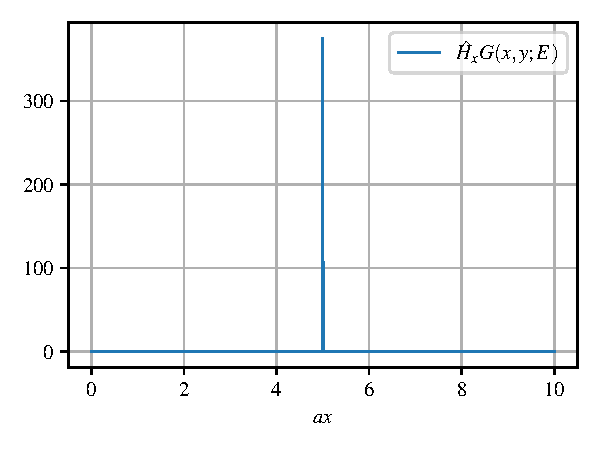
\includegraphics[scale=1]{./figs/checkgreen.pdf}
	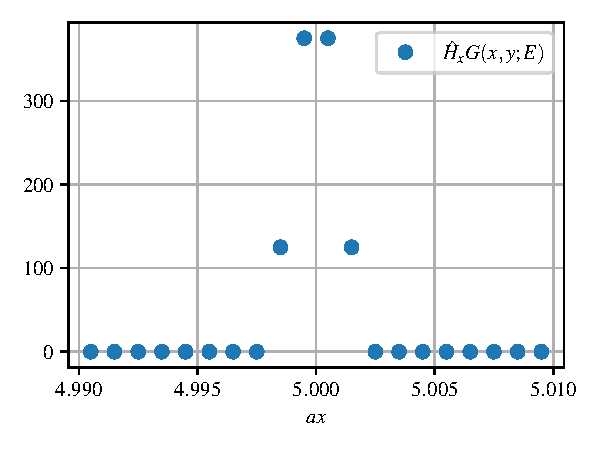
\includegraphics[scale=1]{./figs/checkgreen2.pdf}
	\label{numeric:checkgreen}
	\caption[Green-függvény numerikus ellenőrzése]{Numerikus ellenőrzése \aeqref{green:deltaeq} egyenletnek. A várt eredmény $\delta(x-L/2)$.}
\end{figure}